\documentclass[12pt]{report}
\usepackage{graphicx}
\usepackage{epsfig}
\begin{document}

\begin{center}
{\LARGE\bf Collimator Operation Manual}
\end{center}

\section{\bf Contacts}

\noindent 
Hall-B beam line expert:  

\noindent
Stepan Stepanyan: 269-7196 (office) 584-7196 (pager)

\section{\bf Collimator}

Figure 1 shows the SVT protection collimator. ``3 mm gap'' and ``2 mm gap'' are 1cm-thick Tungsten collimator with a 3 mm gap and 2 mm gap, respectively. ``3 mm gap + Foil'' has a 10$^{-4}$ r.l. Gold foil at the downstream surface. The nominal positions in the collimator coordinate are,

\begin{itemize}
\item
Collimator out:  0 mm
\item
Wire: 20 mm
\item
Middle of 3 mm gap + Foil: 31.5 mm
\item
Middle of 3 mm gap: 54.5 mm
\item
Middle of 2 mm gap: 77 mm
\end{itemize}

\begin{figure}[ht!]
\centering
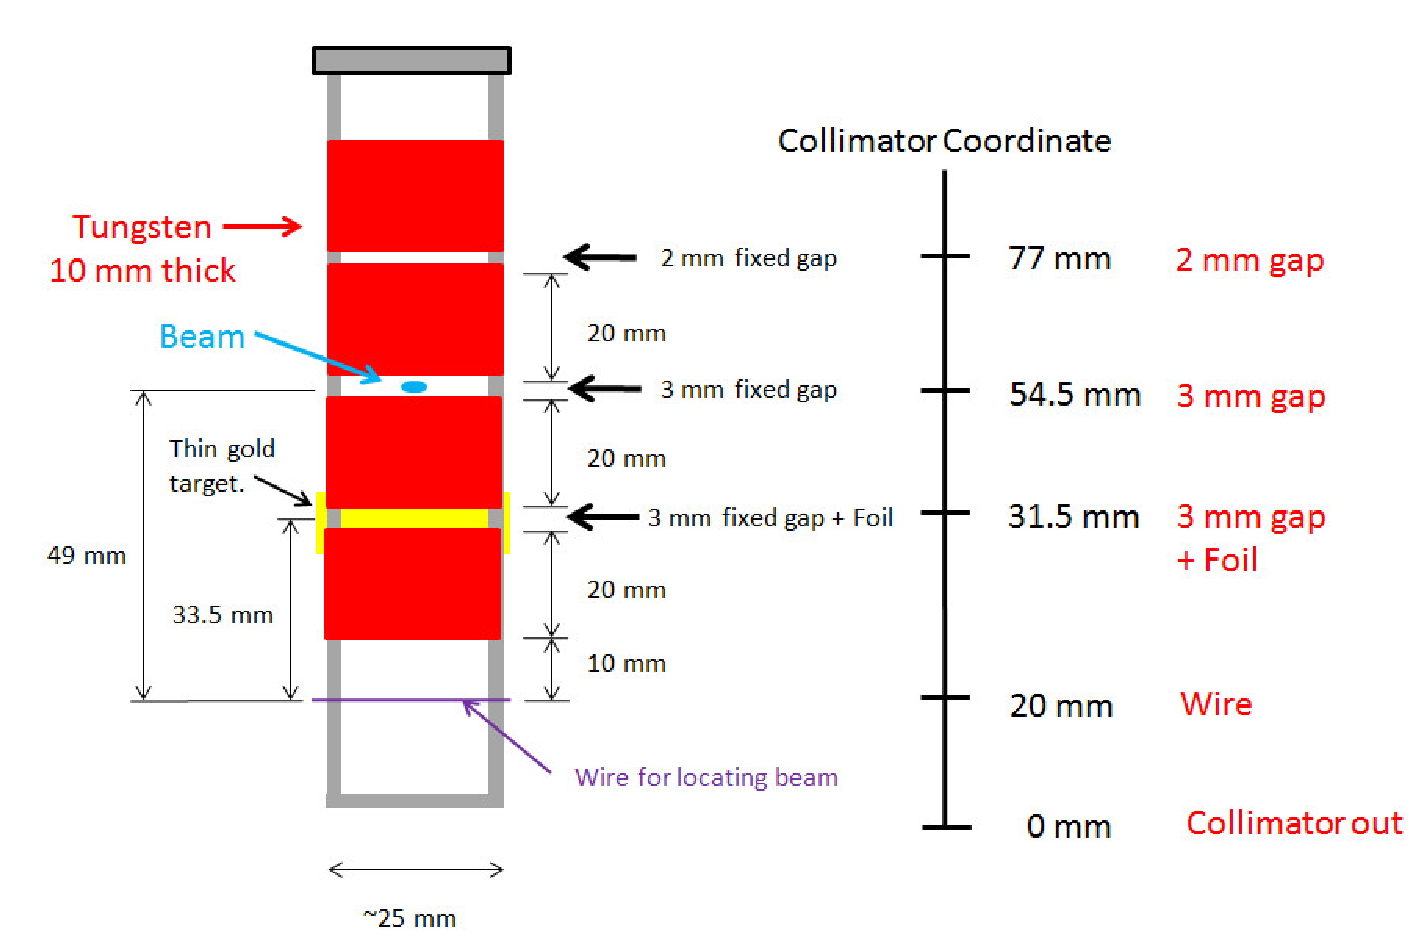
\includegraphics[width=12cm]{CollimatorLadder.eps}
\caption{SVT Protection Collimator}
\label{collimator}
\end{figure}

\section{\bf Wire Scan}

\noindent
{\bf Setup}

\begin{itemize}
\item
MCC is not moving the beam or changing beam conditions
\item
Ask MCC to mask BOM and Downstream Halo Counters in FSD as we are doing Collimator Wire Scan.
\item
SVT is fully retracted and the power is off.
\item
ECal is operational.
\item
Downstream Halo Counter is operational.
\end{itemize}

\noindent
{\bf Scan}

A wire scan can be performed from the wire scan GUI (Figure 2) which is launchable from {\it clas epics}. Once the scan is completed, the collimator will move to ``out'' position.

\begin{itemize}
\item
Type in who you are.
\item
Choose either ECal or Halo Counter as the detector. 
\item
Click ``scan'' using default values.
\item
When the motor is ``Done'', click the red button to the right of ``Analyze Scan Data''.
\item
Find the beam offset ($\Delta$y) from the nominal beam position (y=20 mm).
\end{itemize}

\begin{figure}[ht!]
\centering
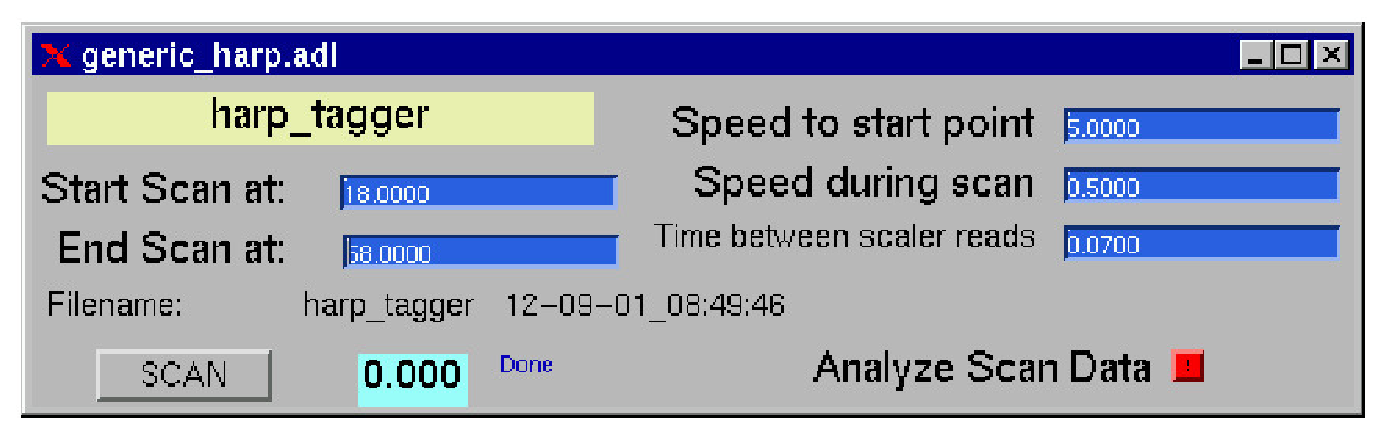
\includegraphics[width=12cm]{harp.eps}
\caption{HARP GUI}
\label{harp}
\end{figure}

\section{Setting the collimator}

Once the beam offset is measured, the collimator can be set by running the collimator GUI shown in Figure 3.

\begin{itemize}
\item
Type in who you are.
\item
Call MCC to turn off the beam and click ``Have you called MCC to turn off the beam?''.
\item
Type in the beam offset value.
\item
Hit ``3 mm + Foil'', ``3 mm gap'', or ``2 mm gap'' button.
\item
Hit ``PANIC'' button to abort.
\end{itemize}

\begin{figure}[ht!]
\centering
\includegraphics[width=12cm]{CollimatorGUI.eps}
\caption{Collimator GUI}
\label{collimator}
\end{figure}

If you don't provide the beam offset, the collimator will be set at the nominal position. If you provide the beam offset and hit ``Reset'', the collimator nominal position will be reset by this value. The collimator position can be fine tuned by providing an arbitrary offset value. However, maximum offset value is limited to 1 mm for the 3-mm gap and 0.5 mm for the 2-mm gap.

Hitting ``OUT'' moves the collimator to y=0 mm.
 
\end{document}
